\documentclass[%
%%% PARA ESCOLHER O ESTILO TIRE O SIMBOLO %(COMENTÁRIO)
%SemVinculoColorido,
%SemFormatacaoCapitulo,
%SemFolhaAprovacao,
%SemImagens,
%CitacaoNumerica, %% o padrão é citação tipo autor-data
%PublicacaoDissOuTese, %% (É também o "default") com ficha catal. e folha de aprovação em branco. Caso tenha lista de símbolos e lista de siglas e abreviaturas retirar os comentários dos arquivos siglas.tex e abreviaturasesiglas.tex. Retirar também os comentários indicados nesse arquivo, nos includes
%PublicacaoArtigoOuRelatorio, %% texto sequencial, sem quebra de páginas nem folhas em branco
%PublicacaoProposta, %% igual tese/dissertação, mas sem ficha catal. e fol. de aprov.
%PublicacaoLivro, %% com capítulos
%PublicacaoLivro,SemFormatacaoCapitulo, %% sem capítulos
english,portuguese %% para os documentos em Português com abstract.tex em Inglês
%portuguese,english %% para os documentos em Inglês com abstract.tex em Português
%,LogoINPE	%% comentar essa linha para fazer aparecer o logo do Governo
,CCBYNC	%% opção de licença
]{tdiinpe}
%]{../../../../../iconet.com.br/banon/2008/03.25.01.19/doc/tdiinpe}

% PARA EXIBIR EM ARIAL TIRAR O COMENT�RIO DAS DUAS LINHAS SEGUINTES
%\renewcommand{\rmdefault}{phv} % Arial
%\renewcommand{\sfdefault}{phv} % Arial

% PARA PUBLICAÇÕES EM INGLÊS:
% renomear o arquivo: abnt-alf.bst para abnt-alfportuguese.bst
% renomear o arquivo: abnt-alfenglish.bst para abnt-alf.bst


%%%%%%%%%%%%%%%%%%%%%%%%%%%%%%%%%%%%%%%%%%%%%
%%% Pacotes já previamente carregados:      %
%%%%%%%%%%%%%%%%%%%%%%%%%%%%%%%%%%%%%%%%%%%%%%%%%%%%%%%%%%%%%%%%%%%%%%%%
%%% ifthen,calc,graphicx,color,inputenc,babel,hyphenat,array,setspace, %
%%% bigdelim,multirow,supertabular,tabularx,longtable,lastpage,lscape, %
%%% rotate,caption2,amsmath,amssymb,amsthm,subfigure,tocloft,makeidx,  %
%%% eso-pic,calligra,hyperref,ae,fontenc                               %
%%%%%%%%%%%%%%%%%%%%%%%%%%%%%%%%%%%%%%%%%%%%%%%%%%%%%%%%%%%%%%%%%%%%%%%%
%%% insira neste campo, comandos de LaTeX %%%
%%% \usepackage{_exemplo_}
% etc.
%%%%%%%%%%%%%%%%%%%%%%%%%%%%%%%%%%%%%%%%%%%%%

%\watermark{Revisão No. ##} %% use o comando \watermark para identificar a versão de seu documento
%% comente este comando quando for gerar a versão final
\usepackage{rotating}
\usepackage{dsfont}
\usepackage{comment}
%%%%%%%%%%%%%%%%%%%CAPA%%%%%%%%%%%%%%%%%%%%%%%%%%%%%%%%
%\serieinpe{INPE-NNNNN-TDI/NNNN} %% n�o mais usado

\titulo{O papel da física de nuvem no acoplamento oceano-atmosfera sobre o Atlântico tropical}
\title{The role of cloud physics on ocean-atmosphere coupling over tropical Atlantic} %% 
\author{Paulo Henrique Santiago de Maria} %% coloque o nome do(s) autor(es)
\descriccao{Tese de Doutorado do Curso de Pós-Graduação em Meteorologia, orientada pelo Dr. Paulo Nobre, aprovada em DD de MÊS POR EXTENSO de 2014.}
\repositorio{aa/bb/cc/dd} %% reposit�rio onde est� depositado este documento - na omiss�o, ser� preenchido pelo SID
\tipoDaPublicacao{TDI}	%% tipo da publica��o (NTC, RPQ, PRP, MAN, PUD, TDI, TAE e PRE) na aus�ncia do n�mero de s�rie INPE, caso contr�rio deixar vazio
\IBI{xx/yy} %% IBI (exemplo: J8LNKAN8PW/36CT2G2) quando existir, caso contr�rio o nome do reposit�rio onde est� depositado o documento

\date{2014}%ano da publica��o

%%%%%%%%%%%%%%%%%%%%%%%%%%VERSO DA CAPA%%%%%%%%%%%%%%%%%%%%%%%%%%%%%%%%%%%%%%%%%%%%%%%
\tituloverso{\vspace{-0.9cm}\textbf{\PublicadoPor:}}
\descriccaoverso{Instituto Nacional de Pesquisas Espaciais - INPE\\
Gabinete do Diretor (GB)\\
Serviço de Informação e Documentação (SID)\\
Caixa Postal 515 - CEP 12.245-970\\
São José dos Campos - SP - Brasil\\
Tel.:(012) 3945-6923/6921\\
Fax: (012) 3945-6919\\
E-mail: {\url{pubtc@sid.inpe.br}}
}

% CEPPII de 09/12/2011 a 08/12/2013:
\descriccaoversoA{\textbf{\ConselhoDeEditoracao:}\\
\textbf{\Presidente:}\\
Marciana Leite Ribeiro - Serviço de Informação e Documentação (SID)\\
\textbf{\Membros:}\\
Dr. Antonio Fernando Bertachini de Almeida Prado - Coordenação Engenharia e Tecnologia Espacial (ETE)\\
Drª Inez Staciarini Batista - Coordenação Ciências Espaciais e Atmosféricas (CEA)\\
Dr. Gerald Jean Francis Banon - Coordenação Observação da Terra (OBT)\\
Dr. Germano de Souza Kienbaum - Centro de Tecnologias Especiais (CTE)\\
Dr. Manoel Alonso Gan - Centro de Previsão de Tempo e Estudos Climáticos (CPT)\\
Drª Maria do Carmo de Andrade Nono - Conselho de Pós-Graduação\\
Dr. Plínio Carlos Alvalá - Centro de Ciência do Sistema Terrestre (CST)\\
\textbf{\BibliotecaDigital:}\\
Dr. Gerald Jean Francis Banon - Coordenação de Observação da Terra (OBT)\\
%Jefferson Andrade Ancelmo - Servi�o de Informa��o e Documenta��o (SID)\\
%Simone A. Del-Ducca Barbedo - Servi�o de Informa��o e Documenta��o (SID)\\
%Deicy Farabello - Centro de Previs�o de Tempo  e Estudos Clim�ticos (CPT)\\
\textbf{\RevisaoNormalizacaoDocumentaria:}\\
Marciana Leite Ribeiro - Serviço de Informação e Documentação (SID) \\
%Maril�cia Santos Melo Cid - Servi�o de Informa��o e Documenta��o (SID)\\
Yolanda Ribeiro da Silva Souza - Serviço de Informação e Documentação (SID)\\
\textbf{\EditoracaoEletronica:}\\
Marcelo de Castro Pazos - Serviço de Informação e Documentação (SID)\\
}

%%%%%%%%%%%%%%%%%%%FOLHA DE ROSTO

%%%%%%%%%%%%%%%FICHA CATALOGR�FICA
%% N�O PREENCHER - SER� PREENCHIDO PELO SID

\cutterFICHAC{Cutter}
\autorUltimoNomeFICHAC{Sobrenome, Nomes} %% exemplo: Fuckner, Marcus Andr�
\autorAbreviadoFICHAC {} %% N�o usado - deixar vazio
\tituloFICHAC{O papel da física de nuvem no acoplamento oceano-atmosfera sobre o Atlântico tropical}
\instituicaosigla{INPE}
\instituicaocidade{São José dos Campos}
\paginasFICHAC{\pageref{numeroDePáginasDoPretexto} + \pageref{LastPage}} %% n�mero total de p�ginas
%\serieinpe{INPE-00000-TDI/0000} %% n�o mais usado
\palavraschaveFICHAC{1.~Palavra chave. 2.~Palavra chave 3.~Palavra chave. 4.~Palavra chave. 5.~Palavra chave  I.~\mbox{Título}.} %% recomenda-se pelo menos 5 palavras-chaves - \mbox{} � para evitar hifeniza��o 
\numeroCDUFICHAC{000.000} %% n�mero do CDU 

% Nota da ficha (para TD)
\tipoTD{Tese} % Disserta��o ou Tese
\cursoFA{Doutorado em Meteorologia}
\instituicaoDefesa{Instituto Nacional de Pesquisas Espaciais}
\anoDefesa{2014} % ano de defesa 
\nomeAtributoOrientadorFICHAC{Orientador}	% pode ser: Orientador, Orientadora ou Orientadores
\valorAtributoOrientadorFICHAC{Paulo Nobre} % nome(s) completo(s)

%%%%%%%%%%%%%%%FOLHA DE APROVA�AO PELA BANCA EXAMINADORA
\tituloFA{\textbf{ATENÇÃO! A FOLHA DE APROVAÇÃO SERÁ INCLUIDA POSTERIORMENTE.}}
%\cursoFA{\textbf{}}
\candidatoOUcandidataFA{}
\dataAprovacaoFA{}
\membroA{}{}{}
\membroB{}{}{}
\membroC{}{}{}
\membroD{}{}{}
\membroE{}{}{}
\membroF{}{}{}
\membroG{}{}{}
\ifpdf

%%%%%%%%%%%%%%N�VEL DE COMPRESS�O {0 -- 9}
\pdfcompresslevel 9
\fi
%%% define em 80% a largura das figuras %%%
\newlength{\mylenfig} 
\setlength{\mylenfig}{0.8\textwidth}
%%%%%%%%%%%%%%%%%%%%%%%%%%%%%%%%%%%%%%%%%%%

%%%%%%%%%%%%%%COMANDOS PESSOAIS
\newcommand{\vetor}[1]{\mathit{\mathbf{#1}}} %% faça as modificações pertinentes no arquivo configuracao.tex

\makeindex  %% não alterar, gera INDEX, caso haja algum termo indexado no texto

\begin{document} %% início do documento %% não mexer

\maketitle  %% não alterar, gera páginas obrigatórias (folha de rosto, ficha catalográfica e folha de aprovação), automaticamente

%%% Comente as linhas opcionais abaixo caso não as deseje
%%%%%%%%%%%%%%%%%%%%%%%%%%%%%%%%%%%%%%%%%%%%%%%%%%%%%%%%%%%%%%%%%%%%%%%%%%%%%%%%%
% Epígrafe %% opcional

\begin{epigrafe} %% insira sua epígrafe abaixo; estilo livre

\hypertarget{estilo:epigrafe}{} %% uso para este Guia
 
\textit{\large``A vida será mais complicada se você possuir uma curiosidade ativa, além de aumentarem as chances de você entrar em apuros, mas será mais divertida''.}

\vspace{1cm}

\hspace{4cm} \emph{\textsc{Edward Speyer}}\\\hspace{4cm} em \textsl{``Seis Caminhos a Partir de Newton''}, 1994

\end{epigrafe}
 %% Opcional
%%%%%%%%%%%%%%%%%%%%%%%%%%%%%%%%%%%%%%%%%%%%%%%%%%%%%%%%%%%%%%%%%%%%%%%%%%%%%%%%%
% Dedicatória %% opcional

\begin{dedicatoria} %% insira sua dedicatória abaixo; estilo livre

\hypertarget{estilo:dedicatoria}{} %% uso para este Guia
 
%% use 'a meus' em vez de 'aos meus', isto é, não use o artigo definido com pronomes possessivos

\newcommand{\mytext}{A meus pais \textbf{Nicanor} e \textbf{Jaci}, à minha irmã \textbf{Luciana} e ao meu esposo \textbf{William}}

%%% sugestão de estilo
\ifcalligra %% fonte calligra presente nas versões mais novas do MiKTeX (>= 2.4)
  \calligra\Large \mytext %% exemplo usando estilo de fonte caligráfica, caso haja
\else
	\itshape\Large \mytext 
\fi

\end{dedicatoria}
 %% Opcional
%%%%%%%%%%%%%%%%%%%%%%%%%%%%%%%%%%%%%%%%%%%%%%%%%%%%%%%%%%%%%%%%%%%%%%%%%%%%%%%%%
% AGRADECIMENTOS %% opcional

\begin{agradecimentos}  %% insira abaixo seus agradecimentos

\hypertarget{estilo:agradecimentos}{} %% uso para este Guia
Agradecemos à MsC Andriana Susana Lopes de Oliveira Campanharo que gentilmente cedeu 
parte dos textos de sua dissertação para este estilo. O original de sua dissertação
encontra-se na Biblioteca Digital do INPE, no endereço \url {http://urlib.net/sid.inpe.br/MTC-m13@80/2006/11.07.12.37}.
Agradecemos também ao Dr. Gerald Jean Francis Banon pelo desenvolvimento e disponibilização deste estilo.
\end{agradecimentos}


 %% Opcional
%%%%%%%%%%%%%%%%%%%%%%%%%%%%%%%%%%%%%%%%%%%%%%%%%%%%%%%%%%%%%%%%%%%%%%%%%%%%%%%%
% RESUMO %% obrigat�rio

\begin{resumo}

%% neste arquivo resumo.tex
%% o texto do resumo e as palavras-chave t�m que ser em Portugu�s para os documentos escritos em Portugu�s
%% o texto do resumo e as palavras-chave t�m que ser em Ingl�s para os documentos escritos em Ingl�s
%% os nomes dos comandos \begin{resumo}, \end{resumo}, \palavraschave e \palavrachave n�o devem ser alterados

\hypertarget{estilo:resumo}{} %% uso para este Guia

%Neste trabalho � analisada a poss�vel natureza ca�tica da turbul�ncia atmosf�rica. As an�lises aqui realizadas, baseadas em dados de temperatura de alta resolu��o, obtidos pela campanha WETAMC do projeto LBA, sugerem a exist�ncia de um comportamento ca�tico de baixa dimens�o na camada limite atmosf�rica. O atrator ca�tico correspondente possui uma dimens�o de correla��o de $D_{2}=3.50\pm0.05$. A presen�a de din�mica ca�tica nos dados analisados � confirmada com a estimativa de um expoente de Lyapunov pequeno mas positivo, com valor $\lambda_{1}=0.050\pm0.002$. No entanto, esta din�mica ca�tica de baixa dimens�o est� associada � presen�a das estruturas coerentes na camada limite atmosf�rica e n�o � turbul�ncia atmosf�rica. Esta afirma��o � evidenciada pelo processo de filtragem por wavelets utilizado nos dados experimentais estudados, que permite separar a contribui��o da estruturas coerentes do sinal turbulento de fundo.

Neste trabalho é avaliado o efeito sobre o acoplamento oceano-atmosfera do oceano Atlântico tropical de alterações no modo como o modelo representa nuvens e convecção.

\palavraschave{%
	\palavrachave{Interação Oceano-Atmosfera}%
	\palavrachave{Representação de Nuvens}%
	\palavrachave{Modelo Acoplado}%
	\palavrachave{Atlântico Tropical}%
	\palavrachave{Temperatura da Superfície do Mar}%
}
 
\end{resumo} %% obrigatório
%%%%%%%%%%%%%%%%%%%%%%%%%%%%%%%%%%%%%%%%%%%%%%%%%%%%%%%%%%%%%%%%%%%%%%%%%%%%%%%%
% ABSTRACT


\begin{abstract}

%% neste arquivo abstract.tex
%% o texto do resumo e as palavras-chave t�m que ser em Ingl�s para os documentos escritos em Portugu�s
%% o texto do resumo e as palavras-chave t�m que ser em Portugu�s para os documentos escritos em Ingl�s
%% os nomes dos comandos \begin{abstract}, \end{abstract}, \keywords e \palavrachave n�o devem ser alterados

\selectlanguage{english}	%% para os documentos escritos em Portugu�s
%\selectlanguage{portuguese}	%% para os documentos escritos em Ingl�s

\hypertarget{estilo:abstract}{} %% uso para este Guia

In this work the possible chaotic nature of the atmospheric turbulence is analysed. The analyses carried out here, based in data of high resolution temperature, obtained from the WETAMC campaign of the LBA project, suggest the existence of a low-dimension chaotic behavior in the atmospheric boundary layer. The corresponding chaotic attractor possess a correlation dimension of $D_{2}=3.50\pm0.05$. The presence of chaotic dynamics in the analysed data is confirmed with the estimate of a small Lyapunov exponent but positive, with value $\lambda_{1}=0.050\pm0.002$. However, this low-dimension chaotic dynamics is associated with the presence of the coherent structures in the atmospheric boundary layer and not to the atmospheric turbulence. This affirmation is evidenced by the process of filtering for wavelets used in the studied experimental data, that allow to separate the contribution of the coherent structures of the turbulent background signal. 

\keywords{%
	\palavrachave{Atmospheric turbulence}%
	\palavrachave{WETAMC campaign}%
	\palavrachave{LBA project}%
	\palavrachave{Chaotic behavior}%
	\palavrachave{Chaotic attractor}%
}

\selectlanguage{portuguese}	%% para os documentos escritos em Portugu�s
%\selectlanguage{english}	%% para os documentos escritos em Ingl�s

\end{abstract} %% obrigatório

\includeListaFiguras %% obrigatório caso haja mais de 3 figuras, gerado automaticamente
\includeListaTabelas %% obrigatório caso haja mais de 3 tabelas, gerado automaticamente

%%%%%%%%%%%%%%%%%%%%%%%%%%%%%%%%%%%%%%%%%%%%%%%%%%%%%%%%%%%%%%%%%%%%%%%%%%%%%%%%%
%abreviaturas e siglas  %% opcional, mas recomendado

\begin{abreviaturasesiglas}  %% insira abaixo suas abreviaturas conforme o modelo.

%% sigla (separador: &--&) significado (quebra de linha: \\)
\\
%WETAMC   &--&   Campanha de Mesoescala Atmosf�rica na Esta��o �mida \\
%IBGE   &--& Instituto Brasileiro de Geografia e Estat�stica\\
%MC    &--&  M�todo das Covari�ncias\\
%EDO   &--&  Equa��es Diferenciais Ordin�rias\\
%EDP   &--&  Equa��es Diferenciais Parciais\\
%ECT   &--&  Energia Cin�tica Turbulenta\\
%FDP   &--&  Fun��o de Distribui��o de Probabilidade\\
%PR    &--&  Plot de Recorr�ncia\\
%FFT   &--&  Fast Fourier Transform \\
%tS1200  &--&  Temperatura medida no n�vel superior �s 12 horas \\
%tS2300  &--&  Temperatura medida no n�vel superior �s 23 horas \\
%tM1200  &--&  Temperatura medida no n�vel m�dio �s 12 horas \\
%tM2300  &--&  Temperatura medida no n�vel m�dio �s 23 horas \\
%tI1200  &--&  Temperatura medida no n�vel inferior �s 12 horas \\
%tI2300  &--&  Temperatura medida no n�vel inferior �s 23 horas \\
%wS1200  &--&  Velocidade vertical do vento medida no n�vel superior �s 12 horas\\
ZCIT &--& Zona de convergência intertropical\\
NEB &--& Nordeste Brasileiro\\

\end{abreviaturasesiglas}
 %% opcional %% altere o arquivo siglaseabreviaturas.tex

%%%%%%%%%%%%%%%%%%%%%%%%%%%%%%%%%%%%%%%%%%%%%%%%%%%%%%%%%%%%%%%%%%%%%%%%%%%%%%%%%
% simbolos

\begin{simbolos}

%% o comando: \hypertarget{estilo:simbolos}{} abaixo � de uso para este Guia
%% e pode ser retirado

\hypertarget{estilo:simbolos}{}
\\
a   &--& primeira contante \\
b   &--& segunda constante \\
$\rho$  &--& densidade de um fluido\\
%$\nu$   &--& viscosidade cinem�tica\\
%$R_{e}$  &--& n�mero de Reynolds\\
$\alpha$  &--& constante de Kolmogorov\\
%$k$ &--&  n�mero de onda\\
$K$ &--&  curtose\\
%$D_{0}$ &--& dimens�o de contagem de caixas\\
%$D_{1}$ &--& dimens�o de informa��o\\
%$D_{2}$  &--& dimens�o de correla��o\\
$\lambda_{1}$  &--& expoente de Lyapunov dominante\\
 

\end{simbolos}

 %% opcional %% altere o arquivo simbolos.tex

\includeSumario  %% obrigatório, gerado automaticamente

\inicioIntroducao %% não altere este comando

%\include{./docs/introducao_corr3} %% 1o capítulo, começo do texto
\chapter{INTRODUÇÃO}

% Visao Geral
A representação das nuvens em modelos climáticos vem se mostrando uma característica crítica na capacidade de reprodução dos padrões observados do clima.

% Justificativa


% Objetivos
\chapter{REVISÃO BIBLIOGRÁFICA}

% Climatologia observacional do atlântico

% Dinamica do acoplamento no atlantico tropical

% Viés dos modelos acoplados

%\section{Descrição observacional da interação oceano-atmosfera sobre o Atlântico tropical}
\section{Ciclo anual climatológico observado no Atlântico tropical}

A Figura~\ref{fig:oisst_act_clim} mostra as médias mensais da temperatura da superfície do mar média entre 16W-4E e 4S-4N, região afetada pela língua fria do Atlântico, obtidas do produto observacional NOAA OISST V2 para o período entre janeiro de 1982 e dezembro de 2013, com os valores para os 32 anos superpostos mês-a-mês. Os valores estão replicados de modo que o ciclo anual se apresenta com uma repetição, permitindo visualização contínua da variação anual em qualquer fase. A linha cinza que conecta meses adjacentes representa a média climatológica mensal fornecendo, portanto, o ciclo anual climatológico.

\begin{figure}[h!]
\centering
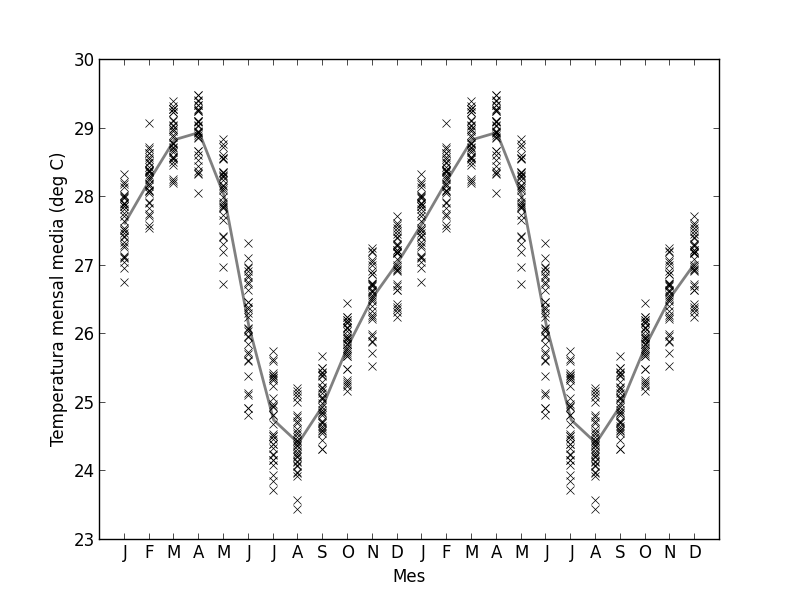
\includegraphics[width=11cm]{figuras/OISST_AtlanticColdTongue.png}
\caption{Médias mensais da temperatura da superfície do mar, média entre $16\,^{\circ}\mathrm{W}$, $4\,^{\circ}\mathrm{E}$ e $4\,^{\circ}\mathrm{S}$, $4\,^{\circ}\mathrm{N}$, referentes ao período entre janeiro de 1982 e dezembro de 2013 do produto NOAA OISST V2.}
\label{fig:oisst_act_clim}
\end{figure}

Pela Figura~\ref{fig:oisst_act_clim} constata-se uma assimetria temporal no ciclo anual, com o resfriamento ocorrendo de forma mais intensa e durando 4 meses, enquanto o aquecimento ocorre durante os 8 meses restantes. \cite{Mitchell/1992}, ao descrever os mecanismos do ciclo anual climatológico da convecção, de TSM e de radiação emitida em onda longa observados na faixa tropical, notando que a maior assimetria entre os hemisférios ocorre em setembro, com máxima penetração dos alíseos de Sul no hemisfério Norte, e quando a língua fria é mais intensa. Para os autores, a língua fria ocorre como consequência da ressurgência equatorial induzida pela tensão superficial do vento de leste que ocorre por causa da convecção sobre as águas mais quentes situadas a oeste. Os autores defendem que que o vento meridional associado às monções sobre os continentes e à ZCIT são instrumentais na efetivação do acoplamento entre atmosfera e oceano e que este acoplamento, por sua vez, é responsável pela proeminência do ciclo anual no setor oeste do cinturão tropical.




%\cite{Mitchell/1992} descrevem o ciclo anual climatológico da convecção e da temperatura da superfície do mar nos trópicos. Para a região do Atlântico, os autores relatam que o ciclo anual, determinado pela marcha do Sol, é o padrão de variabilidade dominante. %variaveis para diagnostico: ROLE, TSM, precipitação, vento.
%\cite{Curtis/1995}, por sua vez, verificam que, durante eventos quentes no Pacífico, 

% figura no formato PDF
% http://stackoverflow.com/questions/8827016/matplotlib-savefig-in-jpeg-format





\subsection{Variabilidade do Atlântico tropical}

\section{Acoplamento oceano-atmosfera no Atlântico tropical: resultados de modelos}
\chapter{MATERIAL E MÉTODOS}



%\include{./docs/turbulencia_e_caos_st_corr6} %% 2o capítulo

%\include{./docs/tecnicas_utilizadas_corr3} %% 3o capítulo

%\include{docs/dados_analisados_corr2} %% 4o capítulo

%\include{docs/analise_e_resultados_corr7} %% 5o capítulo

%\include{docs/conclusoes3} %% 6o capítulo


%% insira quantos capítulos desejar com o seguinte comando:
%\include{_pasta_do_arquivo_/_meu_arquivo_} %%sem a extensão
%% note que deverá haver um arquivo _meu_arquivo_.tex (com extensão) no diretório _pasta_do_arquivo_

%\include{./docs/conclusao}

%% Bibliografia %% não alterar %% obrigatório %testebib
\bibliography{bib/referencia.bib} %% aponte para seu arquivo de bibliografia no formato bibtex (p.ex: referencia.bib)


%\include{./docs/glossario} %% insira os termos do glossário no arquivo glossario.tex %% opcional

\inicioApendice %% opcional, comente esta linha e a seguintes se não houver apendice(s)
%%%%%%%%%%%%%%%%%%%%%%%%%%%%%%%%%%%%%%%%%%%%%%%%%%%%%%
%Apêndice A
\hypertarget{estilo:apendice1}{} %% uso para este Guia
%Este apêndice foi criado apenas para indicar como construir um apêndice no estilo, não existia no original da tese.
%%%%%%%%%%%%%%%%%%%%%%%%%%%%%%%%%%%%%%%%%%%%%%%%%%%%%%
\renewcommand{\thechapter}{}%
\chapter{APÊNDICE A - DESCRIÇÃO DO MODELO ACOPLADO}	% trocar A por B na próxima apêndice e etc
\label{apendiceA}	% trocar A por B na próxima apêndice e etc
\renewcommand{\thechapter}{A}%		% trocar A por B na próxima apêndice e etc

O modelo empregado nas simulações do clima é o BESM 2.4 ...


\section{Componente atmosférica}


\subsection{Representação das nuvens} 


\section{Componente oceânica}

 %% insira apendices tal qual capítulos acima


\inicioAnexo
%%%%%%%%%%%%%%%%%%%%%%%%%%%%%%%%%%%%%%%%%%%%%%%%%%%%%%
%Anexo
%Este anexo foi incluido para explicar como incluir um anexo no estilo, n�o existia no original desta tese.
%%%%%%%%%%%%%%%%%%%%%%%%%%%%%%%%%%%%%%%%%%%%%%%%%%%%%%%%%%%%%%%%%%%%%%%%%%%%%%%%%
\renewcommand{\thechapter}{}%
\chapter{ANEXO A - ABREVIATURA DOS MESES} %% T�tulo do anexo sempre em mai�sculas. Trocar A por B no pr�ximo anexo e etc
\label{anexoA} %% R�tulo aplicado caso queira referir-se a este t�pico em qualquer lugar do texto. Trocar A por B no pr�ximo anexo e etc
\renewcommand{\thechapter}{A}%		% trocar A por B no pr�ximo anexo e etc

\begin{table}[!ht]
 \label{tab:abreviaturas}
  \begin{center}
 	\begin{tabular}{lll}
	 \hline
	  \textbf{Português}    & \textbf{Espanhol}  & \textbf{Italiano}\\ 
   \hline
       janeiro   = jan.   & enero = ene.       & gennaio = gen.\\
       fevereiro = fev.   & febrero = feb.     & febbraio = feb.\\
       março     = mar.   & marzo = mar.       & marzo = mar.\\
       abril     = abr.   & abril = abr.       & aprile = apr.\\
       maio      = maio   & mayo = mayo        & maggio = mag.\\ 
       junho     = jun.   & junio = jun.       & giugno = giu.\\ 
       julho     = jul.   & julio = jul.       & luglio = lug.\\
       agosto    = ago.   & agosto = ago.      & agosto = ago.\\
       setembro  = set.   & septiembre = sep.  & settembre = set.\\
       outubro   = out.   & octubre = oct.     & ottobre = ott.\\
       novembro  = nov.   & noviembre =nov.    & novembre = nov.\\
       dezembro  = dez.   & diciembre = dic.   & dicembre = dic.\\ 
     \hline
   \textbf{Francês}       & \textbf{Inglês}    & \textbf{Alemão}\\
     \hline
       janvier = jan.     & January = Jan.     & Januar = Jan.\\
       %f�vrier = f�v.     & February = Feb.    & Februar = Feb.\\
       %mars = mars        & March = Mar.       & M�rz = M�rz\\
       avril = avr.       & April = Apr.       & April = Apr.\\
       mai = mai          & May = May          & Mai = Mai.\\
       juin = juin        & June = June        & Juni = Juni\\
       juillet = juil.    & July = July        & Juli = Juli\\
       %ao�t = ao�t        & August = Aug.      & August = Aug.\\
       septembre = sept.  & September = Sept.  & September = Sept.\\
       octobre = oct.     & October = Oct.     & Oktober = Okt.\\
       novembre = nov.    & November = Nov.    & November = Nov.\\
       %d�cembre = d�c.    & December = Dec.    & Dezember = Dez. \\ 
    \hline
   \end{tabular}
   \end{center}
%	 \FONTE{Adaptada de \citeonline[p.~22]{NBR6023:2002b}.}
\end{table}
%\include{docs/anexo1}
%\include{docs/anexo2}

\inicioIndice
%%%%%%%%%%%%%%%%%%%%%%%%%%%%%%%%%%%%%%%%%%%%%%%%%%%%%%
%Contracapa
%%%%%%%%%%%%%%%%%%%%%%%%%%%%%%%%%%%%%%%%%%%%%%%%%%%%%%

\thispagestyle{empty}
 \begin{table}
  \begin{center}
  \begin{tabularx}{\textwidth}{X}
   \textbf{PUBLICAÇÕES TÉCNICO-CIENTÍFICAS EDITADAS PELO INPE}
  \end{tabularx} 
  \end{center}
 \end{table}
  
 \begin{table}
  \begin{center}
  \begin{tabularx}{\textwidth}{X X}
      
  \textbf{Teses e Dissertações (TDI)}              & \textbf{Manuais Técnicos (MAN)}\\
\\
Teses e Dissertações apresentadas nos Cursos de Pós-Graduação do INPE.	&
São publicações de caráter técnico que incluem normas, procedimentos, instruções e orientações.\\
\\
\textbf{Notas Técnico-Científicas (NTC)}           & \textbf{Relatórios de Pesquisa (RPQ)}\\
\\
Incluem resultados preliminares de pesquisa, descrição de equipamentos, descrição e ou documentação de programas de computador, descrição de sistemas e experimentos, apresentação de testes, dados, atlas, e documentação de projetos de engenharia. 
&	
Reportam resultados ou progressos de pesquisas tanto de natureza técnica quanto científica, cujo nível seja compatível com o de uma publicação em periódico nacional ou internacional.\\
\\
\textbf{Propostas e Relatórios de Projetos (PRP)}	& \textbf{Publicações Didáticas (PUD)} 
\\
\\
São propostas de projetos técnico-científicos e relatórios de acompanhamento de projetos, atividades e convênios.
&	
Incluem apostilas, notas de aula e manuais didáticos. \\
\\         
\textbf{Publicações Seriadas} 	& \textbf{Programas de Computador (PDC)}\\
\\
São os seriados técnico-científicos: boletins, periódicos, anuários e anais de eventos (simpósios e congressos). Constam destas publicações o Internacional Standard Serial Number (ISSN), que é um código único e definitivo para identificação de títulos de seriados. 
&	
São a seqüência de instruções ou códigos, expressos em uma linguagem de programação compilada ou interpretada, a ser executada por um computador para alcançar um determinado objetivo. Aceitam-se tanto programas fonte quanto os executáveis.\\
\\
\textbf{Pré-publicações (PRE)} \\
\\
Todos os artigos publicados em  periódicos, anais e como capítulos de livros. \\                 \end{tabularx}
  \end{center}
 \end{table}


\end{document}